\chapter{Channels, Pins, and Time Travel}
\label{chap:channels-and-time-travel}

\epigraph{``Those who cannot remember their dependencies are condemned to repeat their compilation errors.''}{--- George Santayana (adapted for sysadmins)}

\noindent
By default, GNU Guix provides thousands of packages in its official repository. But what if you need packages that are not in the main tree, proprietary drivers for your laptop's Wi-Fi card, cutting-edge bioinformatics pipelines, or your company's proprietary microservices?

Welcome to the world of \textbf{Channels}.

\section{What Is a Channel?}

In Guix, a \textbf{Channel} is not an opaque binary PPA or an unverified APT repository. 

A channel is simply a \textbf{Git repository} containing Scheme source files that define packages and services. When you run \guixcmd{guix pull}, Guix clones each channel repository, verifies its cryptographic commit signatures, compiles the Scheme modules, and builds a brand-new \texttt{guix} executable and package database.

\section{Configuring Channels: \texttt{\textasciitilde/.config/guix/channels.scm}}

You configure your active channels by creating a Scheme file at \texttt{\textasciitilde/.config/guix/channels.scm}.

Let us examine a typical multi-channel configuration:

\begin{lstlisting}[style=guixscheme]
;; ~/.config/guix/channels.scm
(list
  ;; 1. The official GNU Guix channel (always required)
  (channel
    (name 'guix)
    (url "https://git.savannah.gnu.org/git/guix.git")
    (branch "master")
    ;; Cryptographic introduction for commit authentication
    (introduction
      (make-channel-introduction
        "9edb3f66fd807b096b48283debd4ddcc33ab9a99"
        (openpgp-fingerprint
          "BBB0 2DDF 2CEA F6A8 0D1D  E643 A2A0 6DF2 A33A 54FA"))))

  ;; 2. Nonguix: Non-free drivers, firmware, and proprietary software
  (channel
    (name 'nonguix)
    (url "https://gitlab.com/nonguix/nonguix")
    (branch "master")
    (introduction
      (make-channel-introduction
        "2a97b46e96194b703221a074ddb4402d5dd99708"
        (openpgp-fingerprint
          "2A39 3FFF 68F4 EF7A 3D29  12AF 6F51 20A0 22FB B2D5"))))

  ;; 3. Guix Science: Scientific software and HPC packages
  (channel
    (name 'guix-science)
    (url "https://codeberg.org/guix-science/guix-science.git")
    (branch "master")
    (introduction
      (make-channel-introduction
        "b3a5e796aa404a60773b06cf317b3e51240366eb"
        (openpgp-fingerprint
          "CA4D 7EB7 5D15 73A8 E426  3850 5F12 30A0 CFFB 97BE")))))
\end{lstlisting}

\section{Notable Custom Channels}

The Guix ecosystem features several essential community channels that expand your package universe:

\begin{itemize}
  \item \textbf{Nonguix}: Provides packages that cannot be included in upstream GNU Guix due to the GNU Free System Distribution Guidelines (FSDG). This includes the vanilla Linux kernel (\texttt{linux}), proprietary Wi-Fi firmware (\texttt{linux-firmware}), Steam, Spotify, Google Chrome, and NVIDIA drivers.
  \item \textbf{Guix Science}: High-Performance Computing (HPC), bioinformatics, computational biology, machine learning (PyTorch, JAX), and computer vision pipelines maintained by academic research institutes worldwide.
  \item \textbf{Guix Past}: A historical channel containing legacy toolchains, GCC 2.95, Python 2.4, and ancient libraries needed to reproduce scientific papers published 15 years ago.
\end{itemize}

\begin{alchemybox}[Channel Authentication with OpenPGP]
Notice the \texttt{introduction} block in each channel definition! Guix uses cryptographic OpenPGP signatures on every single Git commit in a channel. 
If an attacker compromises GitHub or GitLab and pushes a malicious commit without a valid signature from an authorized developer key, \guixcmd{guix pull} will abort with a security failure before executing any code.
\end{alchemybox}

\section{Authorizing Pre-Built Substitutes for Channels}

When using external channels like Nonguix or Guix Science, you don't have to compile large software packages (like the Linux kernel or PyTorch) locally from scratch. Each channel maintains dedicated build farms that serve pre-built binaries (substitutes).

To authorize these substitute servers, add their signing keys and URLs to your system configuration:

\begin{lstlisting}[style=guixcli]
# Download and authorize the Nonguix signing key
wget https://substitutes.nonguix.org/signing-key.pub
sudo guix archive --authorize < signing-key.pub

# Update your Guix daemon with the substitute URL
sudo herd set-substitute-urls guix-daemon \
  https://substitutes.nonguix.org \
  https://bordeaux.guix.gnu.org \
  https://ci.guix.gnu.org
\end{lstlisting}

\section{Channel Pins: Locking Reality}

How do you guarantee that a colleague running \guixcmd{guix pull} gets the exact same package versions you have today?

You \textbf{pin} your channels to specific Git commit hashes:

\begin{lstlisting}[style=guixscheme]
;; Pinned channels.scm for guaranteed reproducibility
(list
  (channel
    (name 'guix)
    (url "https://git.savannah.gnu.org/git/guix.git")
    (commit "a84ef2b9d3e817921a415a77c3e53381a1795c64"))
  (channel
    (name 'nonguix)
    (url "https://gitlab.com/nonguix/nonguix")
    (commit "92e104c8f01bcf5594b2efc8f74f1b8a5b23d9b0")))
\end{lstlisting}

You can generate this pinned configuration automatically from your current system state with:

\begin{lstlisting}[style=guixcli]
guix describe -f channels > channels.scm
\end{lstlisting}

This produces an exact, machine-readable Scheme file representing the precise Git commit hashes of all active channels (\texttt{guix}, \texttt{nonguix}, \texttt{guix-science}).

If you commit that output to a file named \texttt{channels.scm}, anyone can reproduce your multi-channel universe down to the exact bit using \guixcmd{guix time-machine}.

\section{The Superpower: \texttt{guix time-machine}}

Now comes the coup de gr\^ace that makes every other package manager look like an antique.

Suppose you have a \texttt{channels.scm} file containing pins for GNU Guix and Guix Science from three years ago. You want to re-run an experiment today:

\begin{lstlisting}[style=guixcli]
# Run an ad-hoc shell using the exact multi-channel universe from channels.scm
guix time-machine -C channels.scm -- shell python-pytorch r-ggplot2 -- python3 pipeline.py

# Or travel to a specific historic commit on the fly!
guix time-machine --commit=a84ef2b9d3... -- install emacs
\end{lstlisting}

\begin{figure}[htbp]
\centering
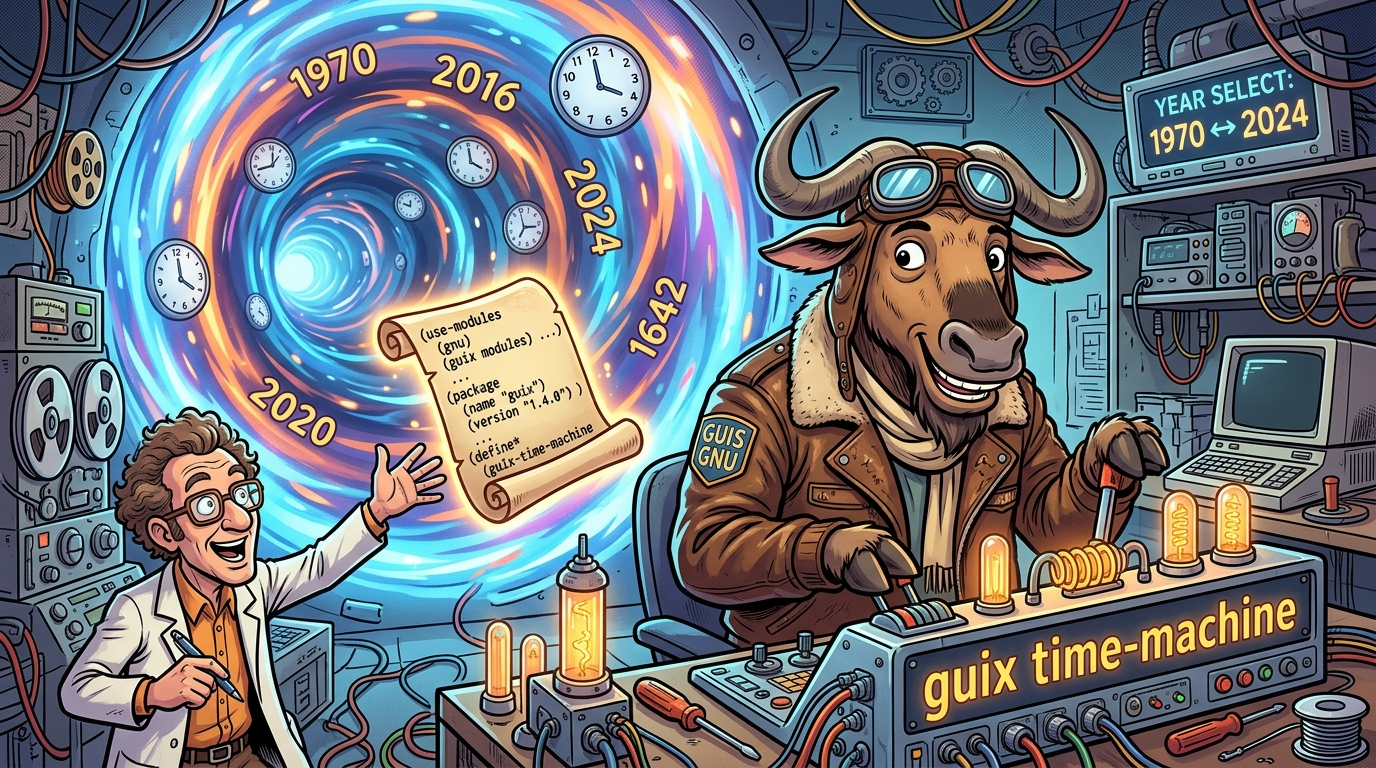
\includegraphics[width=0.92\textwidth]{images/time_machine.jpg}
\caption*{\textit{Figure 3.1: Traveling through the cosmic timeline: \guixcmd{guix time-machine} seamlessly executing 10-year-old scientific code with zero dependency drift.}}
\end{figure}

\begin{tearsbox}[Scientific Reproducibility: A Solved Problem]
In 2016, a survey in \emph{Nature} revealed that over 70\% of researchers had failed to reproduce another scientist's computational experiments due to dependency drift.

With \guixcmd{guix time-machine} and multi-channel pins, scientific pipelines can be re-executed 10 years later producing identical numerical results.
\end{tearsbox}
